\chapter{Podstawy teoretyczne}

Celem rozdziału jest przedstawienie podstawowych definicji, wytłumaczenie aparatu matematycznego oraz metod wykorzystywanych w algorytmach na których skupia się praca. Dodatkowo ma on na celu ułatwienie dalszego czytania poprzez zapoznanie czytelnika z przyjętymi konwencjami, oznaczeniami oraz symbolami, które mogą pojawić się w kolejnych rozdziałach. 


\section{Definicja super-rozdzielczości}

Super-rozdzielczość (ang. Super-Resolution) odnosi się do procesu poprawy rozdzielczości obrazu lub sekwencji obrazów. W kontekście cyfrowym, super-rozdzielczość jest często realizowana za pomocą algorytmów komputerowych, które mają na celu odtworzenie wysokiej rozdzielczości obrazu [Rys \ref{fig:image2}, \ref{fig:image3}] z jednego lub wielu obrazów o niskiej rozdzielczość [Rys \ref{fig:image1}].

\begin{figure}[ht]
    \centering
    \begin{minipage}[t]{0.3\linewidth}
        \includegraphics[width=\linewidth]{Rozdziały/02.Podstawy_teoretyczne/comic.png}
        \caption{Obraz oryginalny}
        \label{fig:image1}
    \end{minipage}
    \hspace{0.5cm}
    \begin{minipage}[t]{0.3\linewidth}
        \includegraphics[width=\linewidth]{Rozdziały/02.Podstawy_teoretyczne/comic_ESRGAN_x4.png}
        \caption{Obraz powiększony czterokrotnie}
        \label{fig:image2}
    \end{minipage}
    \hspace{0.5cm}
    \begin{minipage}[t]{0.3\linewidth}
        \includegraphics[width=\linewidth]{Rozdziały/02.Podstawy_teoretyczne/comic_ESRGAN_x16.png}
        \caption{Obraz powiększony szesnastokrotnie}
        \label{fig:image3}
    \end{minipage}
  \end{figure}


\section{Przegląd metod powiększania obrazów}


Istnieje wiele metod powiększania rozdzielczości obrazów. Najprostszą z nich jest \textbf{interpolacja najbliższego sąsiada}, która polega na powieleniu pobliskich pikseli w celu zwiększenia rozdzielczości obrazu. \\
Metoda ta jest bardzo prosta w implementacji, jednakże nie daje ona zadowalających rezultatów. Obraz powiększony w ten sposób wygląda jak obraz o niskiej rozdzielczości z większymi pikselami [Rys \ref{fig:image5}]. 

\begin{figure}[ht]
    \centering
    \begin{minipage}[t]{0.32\linewidth}
        \includegraphics[width=\linewidth]{Rozdziały/02.Podstawy_teoretyczne/comic.png}
        \caption{Obraz oryginalny}
        \label{fig:image4}
    \end{minipage}
    \hspace{0.5cm}
    \begin{minipage}[t]{0.32\linewidth}
        \includegraphics[width=\linewidth]{Rozdziały/02.Podstawy_teoretyczne/comic_NN_x4.png}
        \caption{Obraz powiększony metodą najbliższego sąsiada}
        \label{fig:image5}
    \end{minipage}
  \end{figure}


Aby poprawić jakość obrazu, można zastosować \textbf{interpolację dwuliniową}. Metoda ta rozszerza interpolację liniową na interpolację funkcji dwóch zmiennych [Rys \ref{fig:image6}]. 

W efekcie polega to na wyznaczeniu średniej ważonej pikseli sąsiadujących z pikselem, który chcemy powielić. Współczynniki wag są wyznaczane na podstawie odległości od piksela, który chcemy powielić.

\begin{figure}[ht]
    \centering
    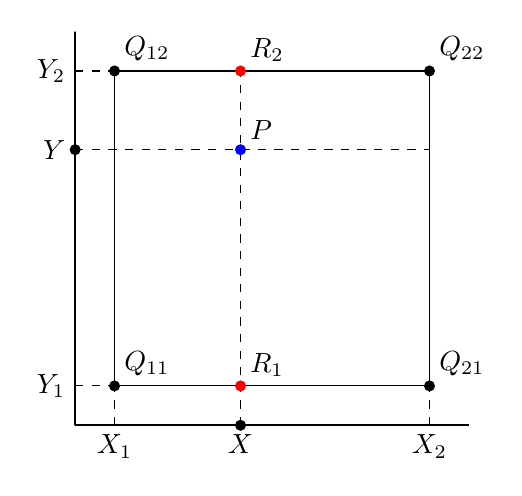
\begin{tikzpicture}[scale=2, dot/.style={circle,fill=black,minimum size=4pt,inner sep=0pt,outer sep=-1pt},]

        % Define the coordinates of the grid points
        \coordinate (A) at (1,1);
        \coordinate (B) at (3,1);
        \coordinate (C) at (1,3);
        \coordinate (D) at (3,3);

        \coordinate (R1) at (1.8,1);
        \coordinate (RY) at (1,2.5);
        \coordinate (R1end) at (1.8,3);
        \coordinate (RYend) at (3,2.5);

        \coordinate (P) at (1.8,2.5);

        \coordinate (X) at (1.8,0.75);
        \coordinate (Y) at (0.75,2.5);
        \coordinate (X1) at (1,0.75);
        \coordinate (X2) at (3,0.75);
        \coordinate (Y1) at (0.75,1);
        \coordinate (Y2) at (0.75,3);
        
        \coordinate (frameS) at (0.75,0.75);
        \coordinate (frameX) at (3.25,0.75);
        \coordinate (frameY) at (0.75,3.25);


        \draw[thick] (frameS) rectangle (frameX);
        \draw[thick] (frameS) rectangle (frameY);
        
        \draw[thin] (A) rectangle (D);
        
        % Draw lines from corners to the interpolated point
        \draw[dashed] (X) -- (R1end);
        \draw[dashed] (Y) -- (RYend);
        \draw[dashed] (X1) -- (A);
        \draw[dashed] (X2) -- (B);
        \draw[dashed] (Y1) -- (A);
        \draw[dashed] (Y2) -- (C);

        % Draw the dots
        \node[dot] at (A) {};
        \node[dot] at (B) {};
        \node[dot] at (C) {};
        \node[dot] at (D) {};
        \node[dot, blue] at (P) {};
        \node[dot, red] at (R1) {};
        \node[dot, red] at (R1end) {};
        \node[dot] at (X) {};
        \node[dot] at (Y) {};
        
        % Labels for the corners
        \node[above right] at (A) {$Q_{11}$};
        \node[above right] at (B) {$Q_{21}$};
        \node[above right] at (C) {$Q_{12}$};
        \node[above right] at (D) {$Q_{22}$};
        
        % Label for the interpolated point
        \node[above right] at (P) {$P$};

        \node[above right] at (R1) {$R_{1}$};
        \node[above right] at (R1end) {$R_{2}$};
        \node[below] at (X) {$X$};
        \node[left] at (Y) {$Y$};
        \node[below] at (X1) {$X_{1}$};
        \node[below] at (X2) {$X_{2}$};
        \node[left] at (Y1) {$Y_{1}$};
        \node[left] at (Y2) {$Y_{2}$};
        

        % Add title
        % \node[below] at (current bounding box.south) {Wizualizacja interpolacji dwuliniowej};

    \end{tikzpicture}
    \caption{Wizualizacja interpolacji dwuliniowej}
    \label{fig:image6}
\end{figure}


\newpage
Kroki algorytmu:
\begin{enumerate}
    \item Przeprowadzana jest interpolacja liniowa wzdłuż osi $O X$:
    
    $$
    \begin{array}{llll}
    f\left(R_1\right) \approx \frac{x_2-x}{x_2-x_1} f\left(Q_{11}\right)+\frac{x-x_1}{x_2-x_1} f\left(Q_{21}\right) & \text { gdzie } & R_1=\left(x, y_1\right), \\ \\
    f\left(R_2\right) \approx \frac{x_2-x}{x_2-x_1} f\left(Q_{12}\right)+\frac{x-x_1}{x_2-x_1} f\left(Q_{22}\right) & \text { gdzie } & R_2=\left(x, y_2\right) .
    \end{array}
    $$
    \item Następnie przeprowadzana jest interpolacja wzdłuż osi $O Y$:
    $$
    f(P) \approx \frac{y_2-y}{y_2-y_1} f\left(R_1\right)+\frac{y-y_1}{y_2-y_1} f\left(R_2\right) .
    $$
\end{enumerate}


W efekcie otrzymujemy obraz wyglądający następująco [Rys \ref{fig:image8},  \ref{fig:image10}].


\begin{figure}[ht]
    \centering
    \begin{minipage}[t]{0.3\linewidth}
        \includegraphics[width=\linewidth]{Rozdziały/02.Podstawy_teoretyczne/bilinear_original.png}
        \caption{Obraz wejściowy}
        \label{fig:image7}
    \end{minipage}
    \hspace{0.5cm}
    \begin{minipage}[t]{0.3\linewidth}
        \includegraphics[width=\linewidth]{Rozdziały/02.Podstawy_teoretyczne/bilinear_enlarged.png}
        \caption{Interpolacja dwuliniowa}
        \label{fig:image8}
    \end{minipage}
\end{figure}

\begin{figure}[ht]
    \centering
    \begin{minipage}[t]{0.35\linewidth}
        \includegraphics[width=\linewidth]{Rozdziały/02.Podstawy_teoretyczne/comic.png}
        \caption{Obraz wejściowy}
        \label{fig:image9}
    \end{minipage}
    \hspace{0.5cm}
    \begin{minipage}[t]{0.35\linewidth}
        \includegraphics[width=\linewidth]{Rozdziały/02.Podstawy_teoretyczne/comic_BILINEARx4.png}
        \caption{Obraz powiększony metodą interpolacji dwuliniowej}
        \label{fig:image10}
    \end{minipage}
\end{figure}


Metoda te daje lepsze rezultaty niż interpolacja najbliższego sąsiada, jednakże wprowadziła ona duże rozmycie, które jest szczególnie widoczne na krawędziach i obszarach wysokiej częstotliwości.


W teorii informacji istnieje koncepcja zwana \textbf{nierównością przetwarzania danych}. Zgodnie z nią niezależnie od sposobu przetwarzania danych, \textbf{nie można dodać informacji, której nie ma w oryginale.} Oznacza to, że brakujących danych nie można odzyskać poprzez dalsze przetwarzanie. Czy to oznacza, że super-rozdzielczość jest teoretycznie niemożliwa? 

Nie, jeśli mamy dodatkowe źródło informacji. 


% \newpage
\section{Wprowadzenie do głębokiego uczenia się w przetwarzaniu obrazów}

Głębokie uczenie rewolucjonizuje przetwarzanie obrazów, wprowadzając modele zdolne do uczenia się cech z serii danych. W przetwarzaniu obrazów, głębokie sieci neuronowe są wykorzystywane do zadań takich jak detekcja obiektów, segmentacja, klasyfikacja obrazów, czy właśnie super-rozdzielczość.

Sieć neuronowa może nauczyć się odtwarzać szczegóły obrazów na podstawie pewnych informacji, które zbiera z dużego zbioru obrazów. 

Szczegóły dodawane do powiększanego obrazu w przy użyciu modelu uczenia maszynowego nie naruszają nierówności przetwarzania danych, ponieważ wykorzystywane informacje są w zbiorze treningowym, nawet jeśli nie ma ich na obrazie wejściowym.






\begin{figure}[ht]
    \centering
    \begin{minipage}[t]{0.3\linewidth}
        \includegraphics[width=\linewidth]{Rozdziały/02.Podstawy_teoretyczne/comic.png}
        \caption{Obraz wejściowy}
        \label{fig:image11}
    \end{minipage}
    \hspace{0.5cm}
    \begin{minipage}[t]{0.3\linewidth}
        \includegraphics[width=\linewidth]{Rozdziały/02.Podstawy_teoretyczne/comic_DWSR_x4.png}
        \caption{Obraz powiększony algorytmem DWSR}
        \label{fig:image12}
    \end{minipage}
    \hspace{0.5cm}
    \begin{minipage}[t]{0.3\linewidth}
        \includegraphics[width=\linewidth]{Rozdziały/02.Podstawy_teoretyczne/comic_ESRGAN_x4.png}
        \caption{Obraz powiększony algorytmem ESRGAN}
        \label{fig:image13}
    \end{minipage}
\end{figure}





\newpage
\section{Wstęp do funkcji falkowych}


Omówienie funkcji falkowych, opis do czego to narzędzie służy począwszy od transformaty Fouriera i jej ograniczeń, 
w jaki sposób funkcje falkowe rozwijają FFT, przedstawienie działania.




